\chapter{Reinforcement Learning y Deep Learning}


\section{Introducción}

En esta sección buscaremos dar una descripción mas detallada, tanto del problema a resolver, como así también de como se aplicaron los conceptos de reinforcement learning y deep learning a las soluciones adoptas durante el desarrollo del mismo. Esta sección no pretende ser una guía o una introducción a reinforcement learning, ni a deep learning, sin embargo es necesario contar con conocimientos básicos de ellos para poder comprender los detalles de la solución propuesta. Dejamos en manos del lector la capacitación en estos a través de los diferentes recursos que pueden hallarse en linea. (ver Capitulo 7 - Bibliografía).
\\\\
Recordemos que el objetivo es desarrollar un agente inteligente, que a partir de un capital inicial, sea capaz de realizar compras y ventas de un activo financiero. El agente no poseerá ningún conocimiento previo acerca del funcionamiento del mercado, ni de la empresa sobre la que opera, ni ningún otro tipo de información. Solo conocerá el precio actual de la acción, y su evolución durante los días previos, junto un conjunto de indicadores bursátiles. 
\\
El agente va a interactuar con un simulador de un mercado bursátil, esta interacción se llevará a cabo siguiendo una serie de acciones, observaciones y recompensas.
Cada interacción será llevada a cabo en episodios que tendrán una duración de m días
\\

\begin{figure}[h!]
	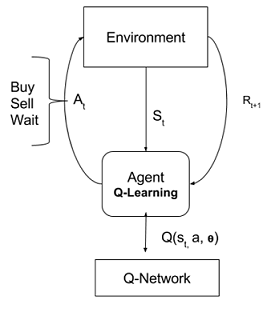
\includegraphics[scale=0.5]{imagenes/deepRLOverview.png}
	\caption{Reinforcement Learning Architecture Overview.}
\end{figure}


En cada instante t, el agente tendrá que seleccionar una acción $a_t$  de un conjunto válido de acciones A = {$a_1, a_2, …, a_n$}. La acción será pasada al entorno, el cual modificará su estado interno y como respuesta a esta interacción el agente recibirá una recompensa $R_{t + 1}$, la cual será calculada por el entorno. El entorno será estocástico, es decir, su comportamiento será no determinístico. Cada uno de los estados contendrá información relevante sobre el papel, como el precio, el volumen, y diferentes indicadores bursátiles, como medias móviles, medias móviles exponenciales, etc.

\section{Configuración de estados}

Ya sea de que se trate de un inversor experimentado o un agente inteligente, difícilmente sea posible tomar una decisión acertada sobre, la compra o venta de un activo, solamente mirando lo que sucede con el precio actual 
del activo, es necesario considerar una ventana de tiempo de tamaño n, para poder analizar la variación que ha tenido y así poder determinar la situación actual del activo, es decir, si se encuentra en una tendencia
alcista o bajista, si se encuentra realizando una corrección de precio o no, si se encuentra en sobre compra o sobre venta, etc. Una manera eficiente de ver esto, es a través, de un gráfico de vela, donde cada vela, representa un periodo, el cual puede ser, un año, una semana, o un mes.

\begin{figure}[h!]
	\centering
	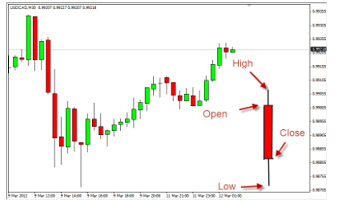
\includegraphics[scale=0.75]{imagenes/candleChart.png}
	\caption{Gráfico de vela.}
\end{figure}

La representación que vamos a adoptar para cada uno de los estados que recibirá el agente, consiste en tomar esta idea de time frame y plasmarla en la estructura de los estados, es decir, el agente será capaz de ver una ventana de tiempo de tamaño n hacia atrás y de diferentes tipos de periodos.

\clearpage

Teniendo en cuenta esto, vamos a definir a cada estado $S_t$  compuesto de 3 capas o layers, de la siguiente forma:
\\\\

$ S_t = L_{dias}, L_{semanas}, L_{meses} \hspace*{1cm} donde \hspace*{0.5cm} L_i = P_1, P_2, ..., P_n $
\\\\
y en donde cada periodo $P_i$ tendrá la siguiente estructura:
\\\\
$P_i$ = Capital\\
\hspace*{0.8cm} Actual Position\\
\hspace*{0.8cm} Open Price\\
\hspace*{0.8cm} Close Price\\
\hspace*{0.8cm} Min Price\\
\hspace*{0.8cm} Max Price\\
\hspace*{0.8cm} Volume\\
\hspace*{0.8cm} ATR\\
\hspace*{0.8cm} MA8\\
\hspace*{0.8cm} EMA20\\
\hspace*{0.8cm} EMA50\\
\hspace*{0.8cm} EMA200\\
\hspace*{0.8cm} RSI\\
\hspace*{0.8cm} DMI\\
\hspace*{0.8cm} MACD\\
\hspace*{0.8cm} BollingerBands\\

\section{Acciones}

En cada instante t el agente podrá decidir comprar, vender o esperar, cada vez que decida comprar o vender, la cantidad de acciones operadas, se calculara en base a una estrategia de entrada y salida del activo pre configurada en el agente.
El agente no tendrá limitación alguna en cuanto a la cantidad de acciones a comprar o vender. Si bien, en la realidad esto no necesariamente seria posible dado que para que pueda comprar una cantidad n a un precio p, debe existir algún vendedor dispuesto a vender n acciones a un precio p cada una.
Ademas cada operación de venta o compra, tendrá un costo asociado c, el cual sera descontado de su capital. El agente no podrá ejecutar la acción elegida si su capital no alcanza para cubrir el costo total de la operación.


\section{El Agente}

Recordemos que el objetivo principal de agente es seleccionar acciones que maximicen su recompensa futura, es decir, deberá de maximizar su capital inicial, para esto vamos a asumir que las recompensa futuras están descontadas por un factor $\gamma$, por cada instante de tiempo t, es decir, vamos a valorizar los rewards más cercanos en el tiempo por un factor $\gamma$. Definimos así el, future discounted reward:
\\\\
\begin{equation}
	 R_t = \sum\limits_{t'= t}^T  \gamma^{t'-t} r_t
\end{equation}

Donde T es el instante en el agente termina de invertir(o bien por qué perdió todo su capital inicial o bien porque se acabaron los datos de simulación).\\
También vamos a definir una función estado-acción óptima, $Q^*(s_t, a_t)$, como la máxima recompensa esperada que podemos alcanzar estando en el estado $s_t$, y seleccionando la acción $a_t$, y luego continuando con una estrategia $\pi$
\\\\
\begin{equation}
Q^*(s, a) = max_{\pi} \E [R_t  |  s_t = s, a_t = a, \pi]
\end{equation}
\\

Esta función tiene una propiedad importante, conocida como Bellman equation, que intuitivamente se basa en lo siguiente: 
Si conociéramos el valor óptimo de $Q^*(s’, a’)$ para el próximo estado s’ y para cada posible acción posible a’, entonces la estrategia óptima de selección de una acción para el estado actual s que maximice la recompensa esperada está dada por
\\\\
\begin{equation}
Q^*(s, a) = max_{\pi} \E_{s' \approx \epsilon} [ r + \gamma max_{a'} Q^*(s', a')  |  s, a]
\end{equation}
\\
La idea general de nuestro algoritmo de aprendizaje va a ser estimar esta función $Q^*$ usando la ecuación de bellman en forma iterativa, esto es:
\\\\
\begin{equation}
Q^*_{i+1}(s, a) = max_{\pi} \E_{s' \approx \epsilon} [ r + \gamma max_{a'} Q_{i}^*(s', a')  |  s, a]
\end{equation}
\\
donde  $i\rightarrow\infty$ y $Q_i \rightarrow Q^*$
\\\\
Esta es la idea detrás del algoritmo de Q-learning que implementará el agente, la cual en principio, parecía suficiente para lograr que el agente aprenda a invertir, sin embargo en la práctica, veremos que en general los estados del mercado no van a repetirse en forma idéntica y que ademas la cantidad de estados posibles hara que sea prácticamente inviable lograr la convergencia hacia $Q^*$.

\section{Q-Network}
Para poder solucionar este inconveniente, vamos a utilizar una función de aproximación, cuyo objetivo será obtener una generalización de los estados, lo cual permitirá en teoría, lograr más rápidamente la convergencia a $Q^*$.\\
Para implementar esta función utilizaremos un red neuronal con con una matriz de pesos $\theta$, inicializada aleatoriamente: 
\\\\
\begin{equation}
Q(s, a, \theta) \approx Q^*(s, a) 
\end{equation}
\\
a la cual denominaremos como Q-network.
Dicha Q-network será entrenada optimizando una función de pérdida L y usando el algoritmo del gradiente descendente.
\\

\begin{equation}
L_i(\theta) = \E_{s, a \approx p(.)}[(y_i - Q(s, a, \theta_i)^2)]
\\\\ 
\end{equation}

\begin{equation}
donde \hspace*{0.5cm}  y_i =  \E_{s \approx \epsilon}[r + \gamma  \hspace*{0.3cm}  max_{a'} Q(s', a', \theta_{i-1}) | s, a]
\end{equation}
\\

Ademas se usara  experience replay para entrenar la Q-Network, es decir, los datos de ejemplos serán generados a partir de la propia experiencia que vaya adquiriendo el agente. Para lograr esto, en cada instante de tiempo t, el agente deberá guardar en un replay memory D, cada experiencia $\epsilon = (s_t, a_t, r_t, s_{t+1})$, observada.
Transcurridos n días el agente deberá ejecutar la fase de entrenamiento de su Q-Network, para esto se generara un mini batch de experiencias pasadas, obtenidas de  su replay memory y con ella se procederá a realizar una última fase actualización de la función de estimación de $Q(s, a, \theta_i)$, usando la regla de actualización de Q-learning y la nueva matriz de pesos $\theta_{i+1}$.


\section{Algoritmo de aprendizaje}

A continuación detallamos el pseudo algoritmo de aprendizaje de nuestro agente.
\\
\\
\begin{algorithm}[1]
\State D $\gets$ new memory\_replay(n)
\State $\theta \gets random() $
\State $Q^*(s, a) \gets Q(\theta)$
\While{$episode \gets generate\_episode() != null$}

\EndWhile
\end{algorithm}

